%hello document


\documentclass[11pt]{article}
\usepackage[top=2.54cm, bottom=2.54cm,left=1.27cm,right=1.27cm]{geometry}
\usepackage{graphicx} 
\usepackage{cite}

\begin{document}

\title{Physics behind the Simulation: A CS296 Report by group 17}
\author{Naveen Sagar\\
120050026 , \texttt{120050026@cse.iitb.ac.in} \\
\and
Prateek Chandan\\
120050042 , \texttt{prateekchandan@cse.iitb.ac.in} \\
\and
Aditya Kumar Akash\\
120050046 , \texttt{adityaakash@cse.iitb.ac.in} \\} 
\date{\today}
\maketitle 

\section{Indroduction}
This document gives details of the assignment report for Lab3 for the course CS296 Software Systems Laboratory, taken by Prof Parag Chaudhary\cite{sir}. 
It contains The details of the new objects added to the Box2D\cite{box2d} simulation, the physics involved behind them, their working along with the image which describes them.  \\
\section{Physics behind the simulation}
This section contains information about the three different objects which is being added to Box2D simulation 
\begin{enumerate}

    \item Conveyer System
    \item The Balanced balls
    \item The Flying Wedge

\end{enumerate}
\subsection{The Conveyer System}
\paragraph{}
A conveyor system\cite{Wiki:1} is a common piece of mechanical handling equipment that moves materials from one location to another. Conveyors are especially useful in applications involving the transportation of heavy or bulky materials. Conveyor systems allow quick and efficient transportation for a wide variety of materials, which make them very popular in the material handling and packaging industries.We have simulated a conveyer system using some rotating wheels.
\paragraph{}
The equation involving the working of Conveyer System:
\begin{eqnarray}
\tau=I*\alpha
\end{eqnarray}
where\par
\begin{description}
  \item $\tau$ is the torque of motor atatched to wheels
  \item I is the moment of Inertia due to mass of wheels and balls
 \end{description}
\paragraph{}
Due to this anglar accleration , a velovity $v$ is achieved by the balls which then moves it to the next conveyer wheel. As the bol reaches to the top or the bottom , dur to the curved surface it rotates and chenges its motion of direction
\begin{figure}[!ht]
    \centering
        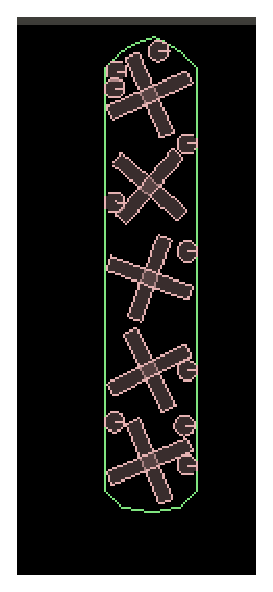
\includegraphics[scale=0.6]{img1.eps}
        \caption{\footnotesize{The image showing Conveyer belt}}
    
\end{figure}

\subsection{The ballanced Balls}
\paragraph{}
Two balls are balanced on a two roattable rods and are balanced by a rod kept in center. The two motors attached rods are kept to push the balls to the upper horizontal shelf which finally moves to open-bucket.
\paragraph{}
The equation involved in balancing:
\begin{eqnarray}
m_1*l_1=m_2*l_2
\end{eqnarray}
where\par
\begin{description}
  \item $l_1$ and $l_2$ are distance of objects from axis of rotation
  \item $m_1$ and $m_2$ are masses of objects
 \end{description}
\paragraph{}
\begin{figure}[!ht]
    \centering
        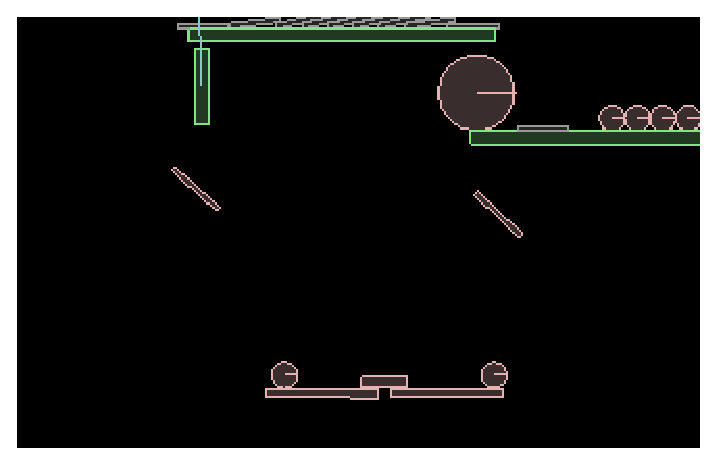
\includegraphics[scale=0.6]{img2.eps}
        \caption{\footnotesize{The image showing The balls which are balanced}}
\end{figure}

\subsection{The Flying wedge}
\paragraph{}
This part simulates the flying away of the light triangular block when the heavy ball falls on it. This happens due to the two inclined wedges which are fixed
\newline
The triangular block moves due to the conservation of momentum
\paragraph{}
The equation for conseravation of momentum\cite{book} is:
\begin{eqnarray}
m_1*v_1+m_2*v_2=m_1*v^f_1+m_2*v^f_2
\end{eqnarray}
where\par
\begin{description}
  \item $v_1$ and $v_2$ are initial velocities of objects
  \item $v^f_1$ and $v^f_2$ are final velocities of objects
  \item $m_1$ and $m_2$ are masses of objects
 \end{description}
\paragraph{}
Due to the final velocity of wedge it mover rigth and then goes up because of the inclined blocks
\begin{figure}[!ht]
    \centering
        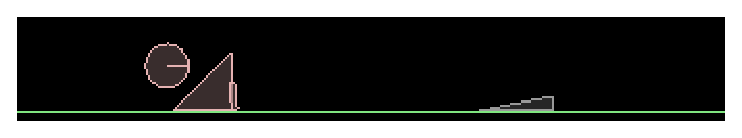
\includegraphics[scale=0.8]{img3.eps}
        \caption{\footnotesize{The image The collision of wedge and the ball}}
\end{figure}

\section{Conclusions}
The objects which are added works properly and follows the laws of ohysics as expected. 
The conveyer system keeps rotating the balls in its system and The rotating wedges and the flying block works as expected\\

\bibliographystyle{plain}

\bibliography{cs296_report_17}

\end{document}

